 \chapter{Design Methodology}
        \section{Methodology}
        \textbf{A. Development of driver circuit} To introduce software based control, microcontroller based actuators modules are to be attached in the power supply lines of the devices (fan and lighting system control).\\
        \textbf{A.1. Study of control methodology} The development of actuator modules designed for each device to be automated will be using plug and play methods so as to convert existing devices into smart ones. The actuators will operate and automate the appliances based on the commands received from the microprocessor.
        \textbf{A.2. Actuator circuit design} \begin{itemize}
        \item \textbf{Incandescent Lamp} The use of pulse width modulated signals that drives a bidirectional control switch i.e., Triac which is connected to the Lamp and thereby with the AC mains. As the width of the PWM is altered the voltage across the lamp will be varied and hence the brightness of the lamp will be controlled.
         \item \textbf{Fans} Speed regulation of fans will be done using the Triac to reduce the energy losses that were occurring by the use of conventional voltage controller. A snubber circuit is connected in parallel with the triac in order to protect it against reverse breakdown.\\
         Now the designed circuit of actuator modules is designed in such a way that there would be no need to interfere with the existing circuitry of the appliances. The existing switches will be simply upgraded by the smart switch boards providing automated control of each appliance over the internet.
        \end{itemize}
        \textbf{B.  Design of the software for the Smart Switch Board}
        The smart switch board needs a central hub for their communication and management. It will receive the inputs from the zero crossing detection circuit and give an optimized output pulse to the switch after processing it using the aforementioned algorithms.\\
        The microcontroller ESP8266 is programmed on NodeMCU platform. The coding is done in C++ language for the microcontroller in order to generate the firing pulses accordingly to operate the driver circuits.\\
         \textbf{C. Development of a user interface to enable user interaction with the system}
         Applications will be developed for the most common mobile platforms, iOS and Android. A cloud-based web app will also be deployed for users to operate from laptops and desktops. The user will be able to use these apps to connect directly to the server hosted on the Home Automation Unit in their homes without any middleware services ensuring their security and privacy.\\
         The programming of the Android Application is done in Java XML. The MQTT broker (CloudMQTT.com) is being used for machine-to-machine internet of things connectivity protocol. It works on a publish/subscribe methodology, and is a lightweight messaging protocol.
        \section{Flow Chart}
        \section{Mathematical analysis and calculations}
        \subsection{Power Supply}
       \begin{equation}
      V_{inp}=230V=V\textsubscript{p} (primary\,voltage) 
      \end{equation} 
      \begin{equation}
       V_{s}(secondary\,voltage)=13.74V
             \end{equation} 
             \begin{equation}
             V_{cp}(peak\,capacitor\,voltage)=13.74*\sqrt{2}-2*0.7 = 18.03V
            \end{equation}
            From the data sheet(attached) of Voltage Regulator(7805), the minimum voltage at the Input Terminal must be above 7V.\\
           As we know the discharging equation of capacitor is :
             \begin{equation}
             V=V_{cp}*e^\frac{-t}{T}
             \end{equation}
            \begin{equation}
            7=18.03*e^\frac{-5*10^{-3}}{T}
             \end{equation}
             By Solving,
             \begin{equation}
             T=5.28ms
             \end{equation}
              \begin{equation}
             R*C=5.28ms
             \end{equation}
             From Diode Bridge Rectifier,
              \begin{equation}
             V(drop)=1.4V=I*R
             \end{equation}
              \begin{equation}
            I=500mA(load\,current)
             \end{equation}
       	By solving, 
       	\begin{equation}
             R=2.8{\si{\ohm}}
             \end{equation}
             Putting in eqn 3.7,
             \begin{equation}
             C=1880{\si\micro}F
             \end{equation}
             So, we have used slightly larger value of capacitor i.e. 2200{\si\micro}F.
             \subsection{Zero Crossing Circuit}
             From data sheet(attached) of A4N25 Transistor based Octocoupler:
             For internal Diode to turn ON -
             \begin{equation}
             I(max.\,permissible\,limit)=60mA
             \end{equation}
             \begin{equation}
            Rectified\,Voltage,V=5.21V
             \end{equation}
             \begin{equation}
            R_{connected}=165{\si\ohm}
             \end{equation}
             \begin{equation}
             I_{actual}=\frac{V}{R_{connected}}=31.57mA
             \end{equation}
             We have connected two resistors each of 330{\si\ohm} in parallel for protection purpose.So, power loss across each resistor is :
             \begin{equation}
            P_L=I^2*R={(15.78*10^{-3})}^2*330=82.22mW<500mW
             \end{equation}
             Thus, the resistor will remain safe. 
             \subsection{Triac Circuit}
             From the Triac Circuit,
             \begin{equation}
            V_{0\,rms}=\sqrt{\frac{1}{2{\pi}}(\int^{\pi}_{\alpha}{{(V_msin\theta)}^2}d\theta+\int^{2\pi}_{\alpha+\pi}{{(V_msin\theta)}^2}d\theta}
             \end{equation}
            On solving, the output rms voltage of Triac is:
            \begin{equation}
            V_{0\,rms}=\frac{V_m}{\sqrt{2}}[\sqrt{\frac{1}{\pi}((\pi-\alpha)+\frac{sin2\alpha}{2})}]
             \end{equation}
             Now, for different firing angle, the output voltage across load would be different as:
             for $\alpha$=0$^\circ$
             \begin{equation}
             V_{o\,rms}=\frac{V_m}{\sqrt{2}}
             \end{equation}
             for $\alpha$=30$^\circ$
             \begin{equation}
            V_{o\,rms}=\frac{V_m}{\sqrt{2}}*0.98
             \end{equation}\
             \& so on...
             \subsection{Optocoupler}
             From datasheet of MOC3041 Optocoupler:
             \begin{equation}
             I(max.\,permissible\,limit)=60mA
             \end{equation}
             Now, \\
             \begin{equation}
             Voltage\,applied,V=3.3V
             \end{equation}
             Hence,
             \begin{equation}
             R_{reqd.}=\frac{V}{I}=\frac{3.3V}{60mA}=55{\si\ohm}
             \end{equation}
             Now, we have connected two resistors(120R, 100R) so that the power rating of resistors do not exceed. 
             Now,
             \begin{equation}
             P_L(R_1=120R)=I^2*R=(27mA)^2*120{\si\ohm}=89.25mW<500mW
             \end{equation}
             Similarly,
             \begin{equation}
             P_L(R_2=100R)=I^2*R=(33mA)^2*100{\si\ohm}=108.9mW<500mW
             \end{equation}
             So, resistors will remain safe.
             \subsection{Ac Fan}
             From datasheet(attached) of ac axial fan:
             \begin{equation}
            L=3H,\,R=1.67K{\si\ohm}
             \end{equation}
             So,
             \begin{equation}
             X_L=w*L=3*2\pi*50=942.477
             \end{equation}
             \begin{equation}
             tan{\theta}=\frac{X_L}{R}
             \end{equation}
             \begin{equation}
             \theta=tan^{-1}(\frac{X_L}{R})
             \end{equation}
             \begin{equation}
             \theta=tan^{-1}(\frac{94204777}{1.67*1000})
             \end{equation}
             \begin{equation}
             \theta=29.43^\circ
             \end{equation}
             Now, for the circuit to start operating-\\
             \begin{equation}
             Firing\,angle(\alpha)>=\theta 
             \end{equation}
             Hence,
             \begin{equation}   
             \alpha>29.43^\circ
             \end{equation}
               
        \section{Circuit Diagram}
        	\begin{figure}[h!]
        		\includegraphics[width=\textwidth]{photos/ckt-dgm/5VDCPowerSupply.jpg}
        		\caption{5V DC Power Supply}
        	\end{figure}
	        \begin{figure}[h!]
	        	\includegraphics[width=\textwidth]{photos/ckt-dgm/ZeroCrossingCircuit.jpg}
	        	\caption{Zero Crossing Detection Circuit}
	        \end{figure}
		    \begin{figure}[h!]
		    	\includegraphics[width=\textwidth]{photos/ckt-dgm/LightDimmerCircuit.jpg}
		    	\caption{Triac based Dimmer Circuit}
		    \end{figure}
        \section{Hardware Design}
	        \begin{figure}[h!]
	        	\includegraphics[width=\textwidth]{photos/hardware/PCBDesign.jpg}
	        	\caption{PCB Layout for the design}
	        \end{figure}
		  
        \section{Hardware System}
	        \begin{figure}[h!]
	        	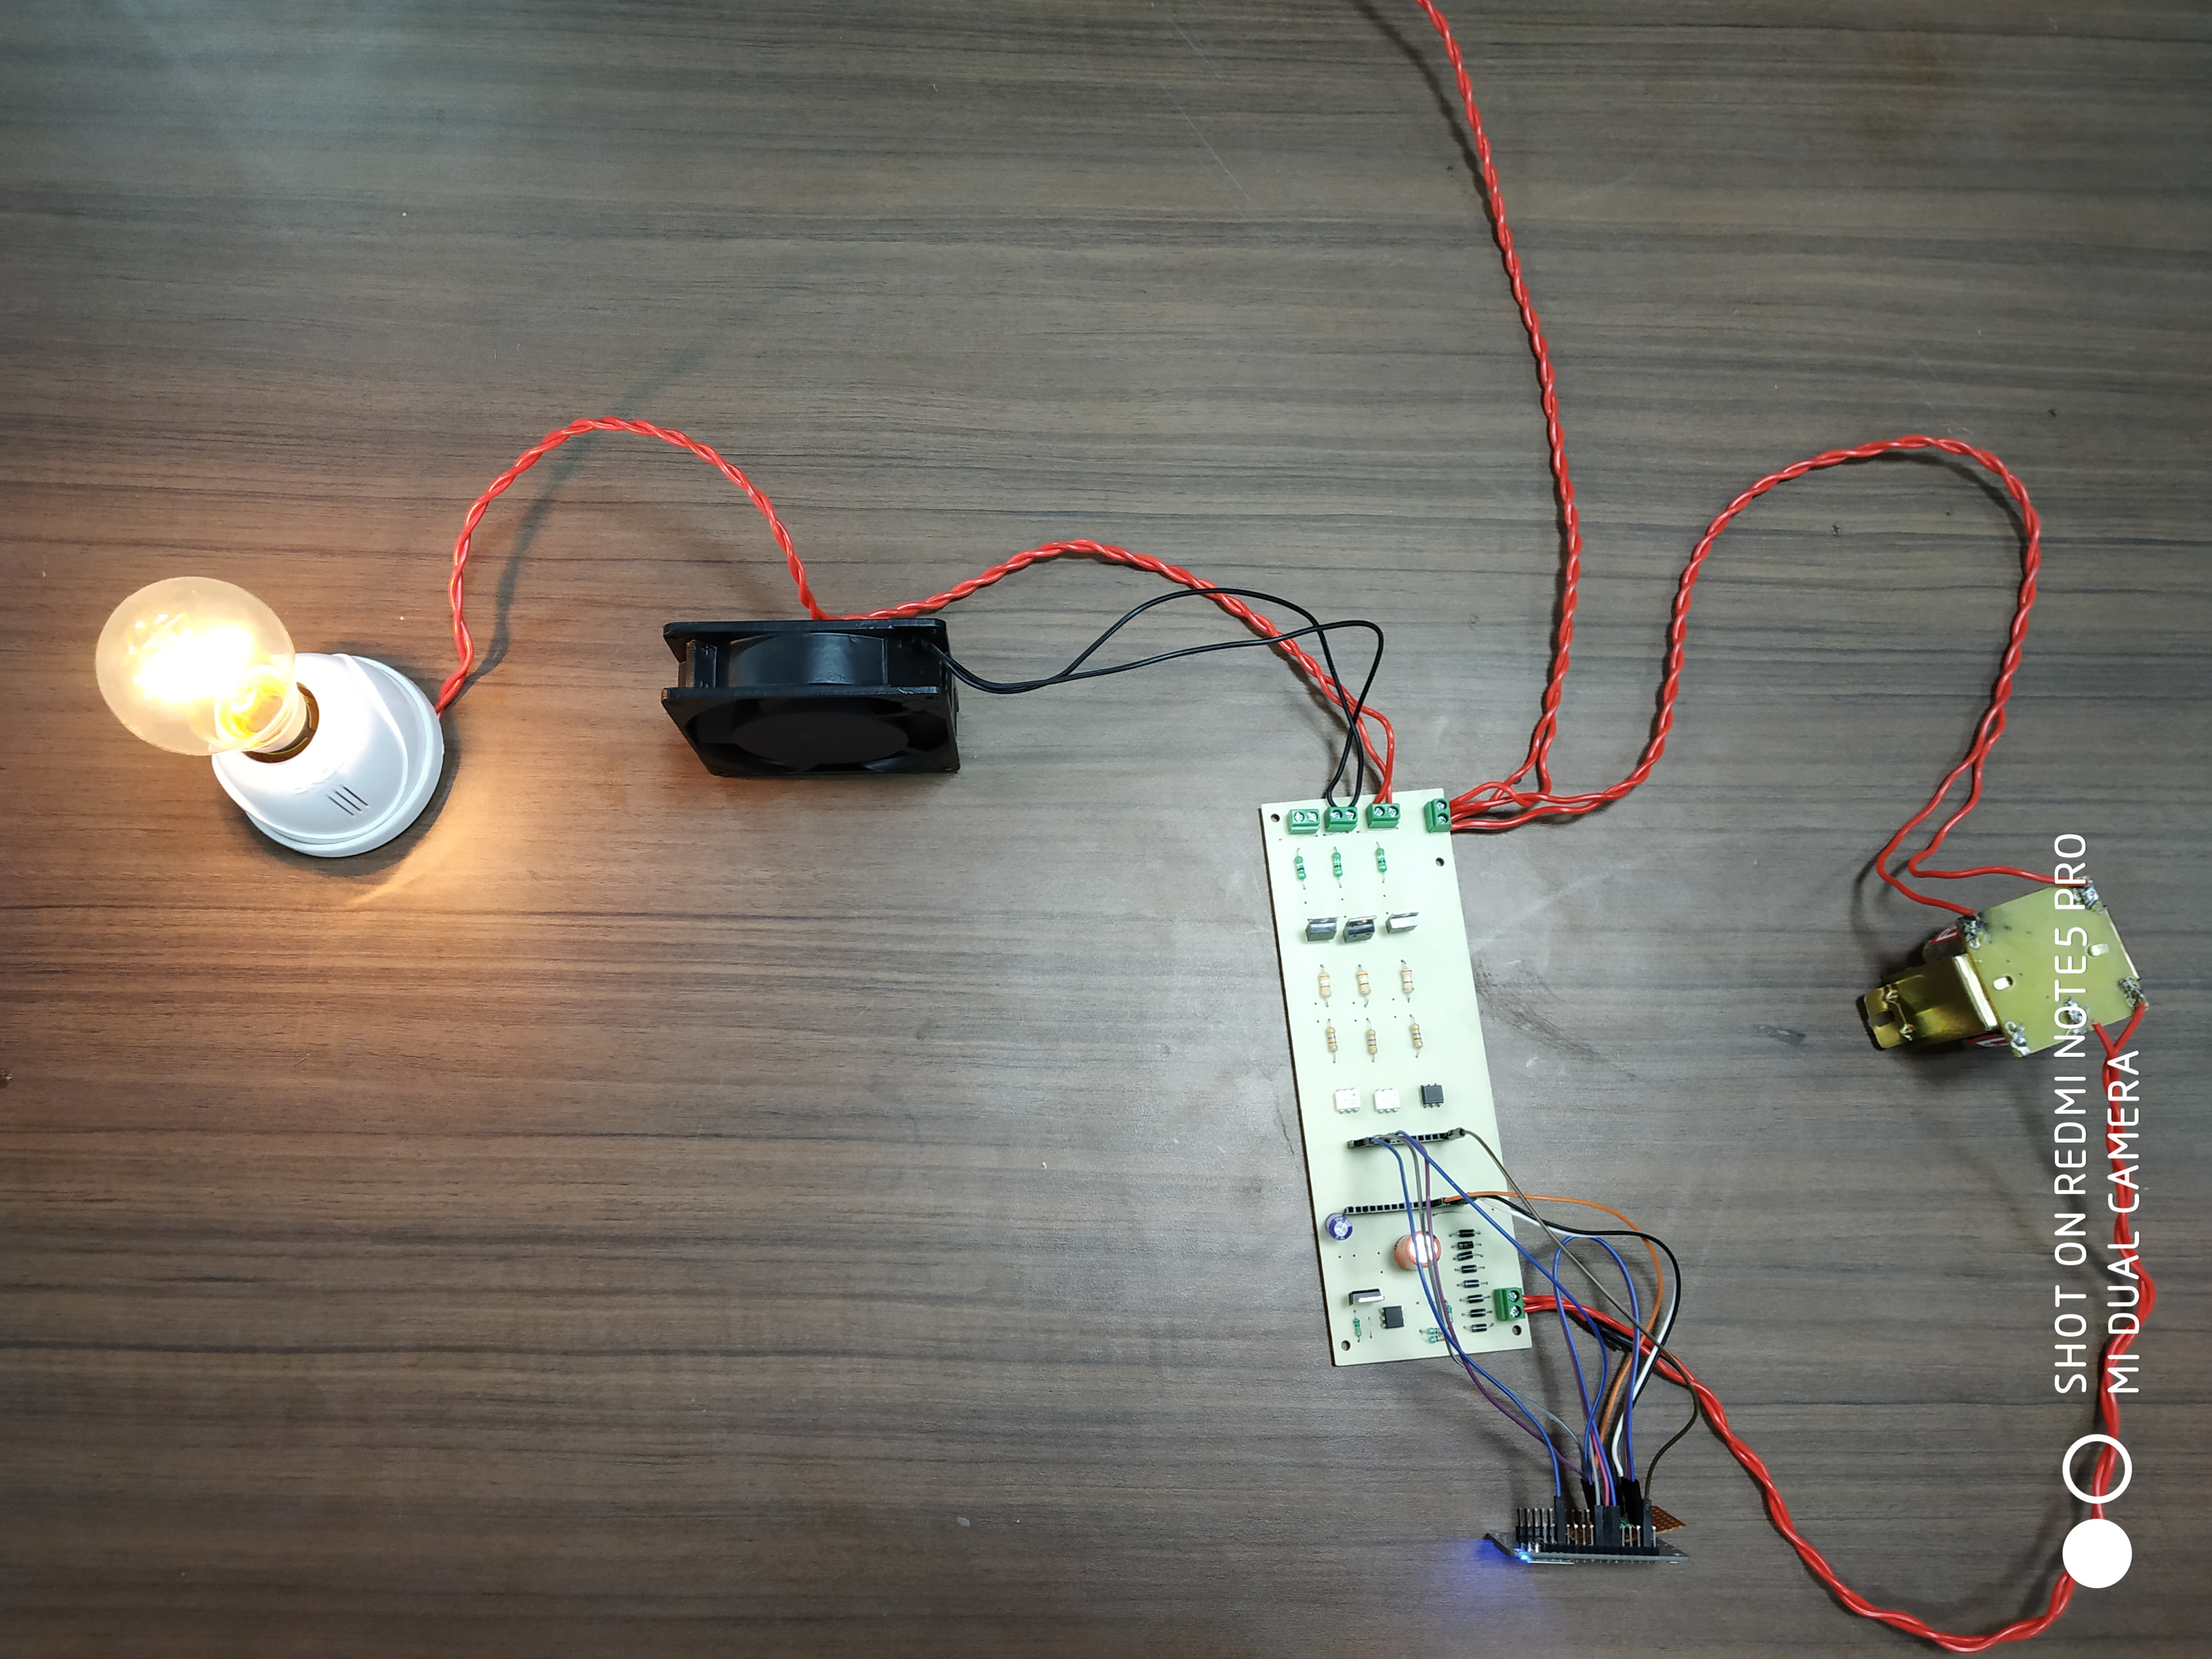
\includegraphics[width=\textwidth]{photos/hardware/Working1.jpg}
	        	\caption{Demonstration of the complete project}
	        \end{figure}

			\begin{figure}[h!]
				\includegraphics[width=\textwidth]{photos/hardware/Working3.jpg}
				\caption{Demonstration of the complete project}
			\end{figure}  